m\section{Measurements}

\subsection{Measuring the magnetic field}
\paragraph{We measured the magnetic} 
field inside the hole for the probe with the Hall effect sensor described in the setup section. 
The sensor was initialized for $B = 0$ mT before the measurement. We first measured over the 
entire range accessibile for a constant current $I$. Results are shown in table \ref{tab:b_height}. 
The height $z$ is measured from the point where the hole for the probe ends above. 
Not all the collected data is displayed, as the linear dependence is shown already by a subset. Further 
the dependency on $U$ is not displayed, as the magnetic field induced electrically only depends on the 
$I$. The uncertainty $s_B = 5$ mT was chosen because of fluctuations over time, especially a 
downshift in magnetic field and current in time, being clearly connected to the rising resistance with 
increasing temperature of the coil. $s_z = 0.4$ is the accuracy allowed by the scale fixed to the 
Hall effect sensor. A possible offset both for $B$ and $z$ cannot be excluded. At least in the latter case, 
the consequences would be very small, as the working point is quite large and the homogenity, which 
in this case could still be shown, is of much higher importance. 
\begin{table}[htdp]
\centering
    \begin{tabular}{|p{1.34cm}|p{2.16cm}|p{0.8cm}|p{1.34cm}|p{2.16cm}|p{0.8cm}|p{1.34cm}|p{2.16cm}|}
        \cline{1-2}\cline{4-5}\cline{7-8}
        $z$ / mm \cellcolor{LightCyan}& $B$ / mT \cellcolor{LightCyan}&&
        $z$ / mm \cellcolor{LightCyan}& $B$ / mT \cellcolor{LightCyan}&&
        $z$ / mm \cellcolor{LightCyan}& $B$ / mT \cellcolor{LightCyan}\\ 
        \cline{1-2}\cline{4-5}\cline{7-8}
        0 & 228 &&14 & 349 &&26 & 349 \\ 
        3 & 341 &&15 & 349 &&27 & 349 \\ 
        4 & 346 &&16 & 350 &&28 & 349 \\ 
        5 & 348 &&17 & 350 &&29 & 349 \\ 
        6 & 349 &&18 & 350 &&30 & 349 \\ 
        7 & 350 &&19 & 350 &&31 & 349 \\ 
        8 & 350 &&20 & 350 &&32 & 348 \\ 
        9 & 350 &&21 & 350 &&33 & 348 \\ 
        10 & 350 &&22 & 350 &&34 & 347 \\ 
        11 & 349 &&23 & 350 &&35 & 347 \\ 
        12 & 349 &&24 & 349 &&36 & 346 \\ 
        13 & 349 &&25 & 349 &&37 & 345 \\ 
        \cline{1-2}\cline{4-5}\cline{7-8}
    \end{tabular}
    \caption{
        Measurement of unmodulated magnetic field $B$ at height $z$ for $I = 2.62$ A.Corresponding uncertainties: $\Delta z = 0.4$ mm, $\Delta B = 5$ mT.
        }
    \label{tab:b_height}
\end{table}

 
\paragraph{Then, we measured} 
the dependency of $B(I)$ in a broader range of $I \in (0.57 2.58)$ A 
and for a smaller range, closer to the suspected region of resonance 
for the given HF generator (table \ref{tab:b_I}). A third measurement at small scale 
but higher current $I > 3.45$ A is not displayed, as this region will not be under 
concern in the evaluation (see appendix \ref{sec:appendix}). 
\begin{table}[htdp]
\centering
    \begin{tabular}{|p{1.34cm}|p{2.16cm}|p{0.8cm}|p{1.34cm}|p{2.16cm}|}
        \cline{1-2}\cline{4-5}
        $I$ / A \cellcolor{LightCyan}& $B$ / mT \cellcolor{LightCyan}&&
        $I$ / A \cellcolor{LightCyan}& $B$ / mT \cellcolor{LightCyan}\\ 
        \cline{1-2}\cline{4-5}
        0.57 & 89 &&2.48 & 346 \\ 
        0.86 & 127 &&2.50 & 348 \\ 
        1.29 & 183 &&2.52 & 350 \\ 
        1.74 & 242 &&2.54 & 352 \\ 
        2.13 & 291 &&2.56 & 354 \\ 
        2.58 & 348 &&2.58 & 355 \\ 
        2.89 & 405 &&2.58 & 357 \\ 
        3.36 & 442 &&2.60 & 359 \\ 
        3.88 & 474 &&2.62 & 361 \\ 
        4.30 & 497 &&2.64 & 365 \\ 
        4.72 & 516 &&2.66 & 365 \\ 
        5.11 & 530 &&2.68 & 367 \\ 
        \cline{1-2}\cline{4-5}
    \end{tabular}
    \caption{
        Measurement of magnetic field $B$ for current $I$ at height $z = 2$ cm. Corresponding uncertainties: $\Delta I = 0.01$ A, $\Delta B = 5$ mT.
        }
    \label{tab:b_I}
\end{table}

\FloatBarrier

\subsection{Direct measurement of resonance frequency}
\paragraph{In this section}, 
we give an overview over the direct measurements of the resonance frequency
for the different probes. The first part of this measurement was dominated by difficulties 
to find the absorption peaks, as the signal we observed on the oscilloscope was quite noisy. 
Only after a long time searching and further support of our tutor did we find any absorption 
peaks at all. This is due to several problems of rather technical nature:
\begin{itemize}
    \item
        The fine tuning of the frequency was not possible to the necessary degree (only
        steps of $0.05$ MHz possible). Once specified, the frequency was quite stable, though, 
        with fluctuations of $\Delta f_{HF} = \pm 0.0001$ MHz (last displayed digit).
    \item
        As a consequence we relied on fine tuning the 
        current and with it the underlying (constant) magnetic field of the main coil. 
        Even this tuning was not easy and limitied to a degree of exactness which 
        allowed only to find \emph{a} signal of absorption. Absorption was seen only in 
        a range of $\Delta I < 0.01$ A, thus smaller than the last digit displayed and 
        corresponding to roating the potentiometer by the lowest angles possible using our hands. 
    \item
        Very shortly after finding the signal, it disappeared again.
        Contrary to our expectations prior to the experiment, 
        we were not able to get a more exact 
        value of $f_R$ by trying to get equidistant absorption peaks. 
        We obtained the data displayed below by saving a 'single run' of the 
        oscilloscope right after the absorption signal was noticed. 
    \item 
        Analogously to the measurements of the section above, we saw the current dropping 
        over time while the voltage remained stable withing the displayed digits. 
        The rate of dropping can be specified by approximately 
        \begin{equation}
            \frac{\Delta I }{\Delta t} = \frac{0.01 \, \A}{10 \, \mathrm{min}} \, .
        \end{equation}
    \item
        We got a much more pronounced signal for small amplitudes of the HF oscillation. 
        However, this amplitude was very unstable close to it's minimum. Many times, it would 
        drop below the threshold of generating a signal at all, so that we had to readjust the 
        corresponding potentiometer constantly. Only the later measurements during the second day 
        of measuring could be achieved at a higher and more stable amplitude. 
\end{itemize}
The collected data was recorded in form of the signal measured by the oscilloscope. 
Due to the described instabilities, we made all recordings right after finding a signal. 
Several seconds later, there was no more signal observed.
We show the input signal given by the sine modulation of the external $B$-field and 
the correlated absorption signal in the figures below. Figure \ref{fig:f_r_F} shows 
some of the measured absorption peaks for fluor, either as a fluid or in Teflon. 
One can observe that the number of peaks does not coincide with the number of zero 
intersects of the $B$-modulation, which is shown on the bottom of the figure. 
However, the measured frequency and corresponding can still be used for further calculations, 
keeping in mind appropriate errors. 
As seen in figures \ref{fig:f_r_H} and \ref{fig:f_r_glycol}, the same is true for 
the measurements of the proton of $^1$H in water and in glycol. For the measurements with 
water, glycole, Teflon and the last measurement of the fluid fluor, we measured the $B$-field 
directly. We estimate the uncertainties to be $s_B = 5$ mT due to the fluctuations seen before and 
$s_{\nu_r} = 0.0001$ MHz, the last digit displayed. 
Choosing the last measurement for fluid fluor and one arbitrary for the other three samples, we get the 
following pairs of resonance frequency $\nu_r$ and measured 
$B$-field, shown in table \ref{tab:f_r}. 
We did not use the linear fit, since we already observed the nonlinear behavior and 
made separate measurements for $B$ right after finding the absorption signal. 
\renewcommand{\arraystretch}{1.5}
\begin{table}[htdp]
\centering
\begin{tabular}{|p{6.18cm}|p{3.82cm}|p{3.82cm}|}
        \hline
        \rowcolor{LightCyan}
        Sample & $B_\mathrm{measured}$ / mT & $\nu_r$ / MHz\\ \hline
        $^{19}$F, fluid & 419 & 18.6905\\
        $^{19}$F, Teflon & 423 & 18.68130\\
        $^1$H   & 395 & 16.8503 \\
        Glycol  & 394 & 16.8704 \\
        \hline
    \end{tabular}
    \caption{
        Measured pairs of $B$ and resonance frequency $\nu_r$ for all four samples with the direct measurement 
        of the absorption peaks. The uncertainties are estimated by $s_B = 5$ mT 
        and $s_{\nu_r} = 0.0001$ MHz. 
        }
    \label{tab:f_r}
\end{table}
\begin{figure}
	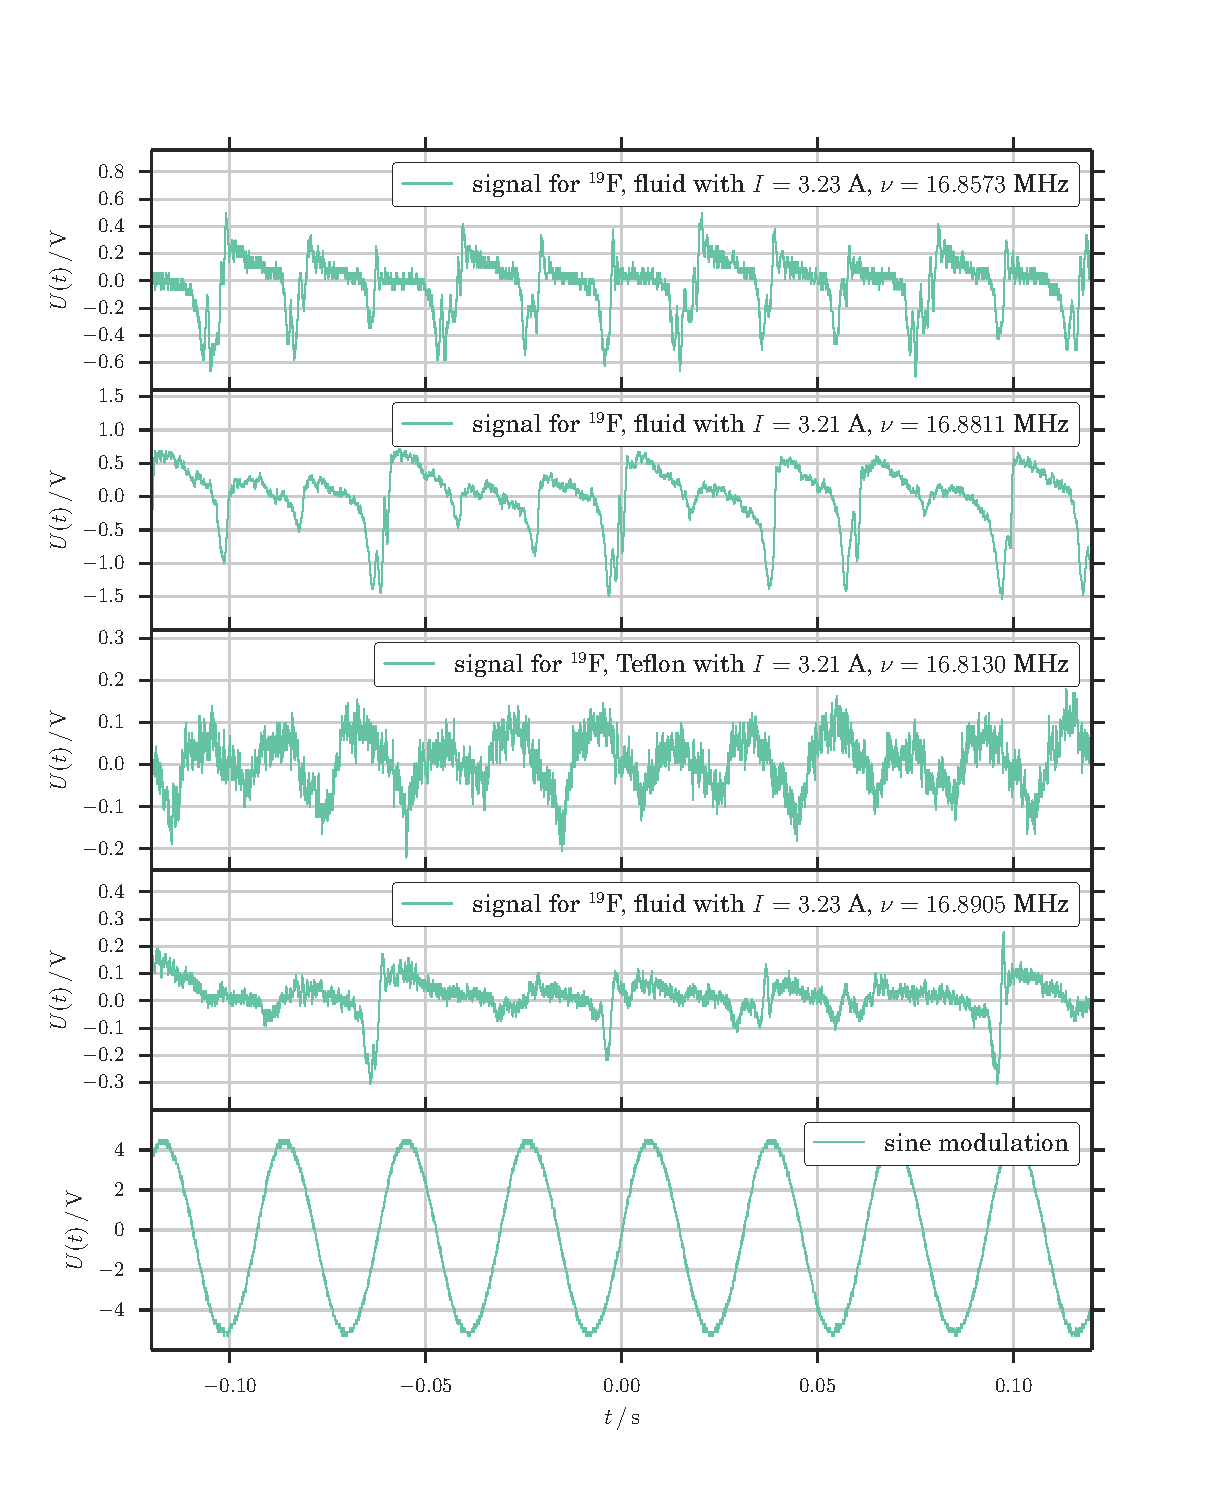
\includegraphics[width=\textwidth]{figures/f_r_F.pdf}
	\caption{
		Absorption peaks of $^{19}$F, measured 
		at four different times. One can observe absorption peaks in each of
		the measured signals. However, due to the described problems with fine tuning,
		we were not able to produce equidistant peaks with a distance of half the,
		wavelength of the input signal, shown in the lowest graph.
		}
	\label{fig:f_r_F}
\end{figure}

\begin{figure}
	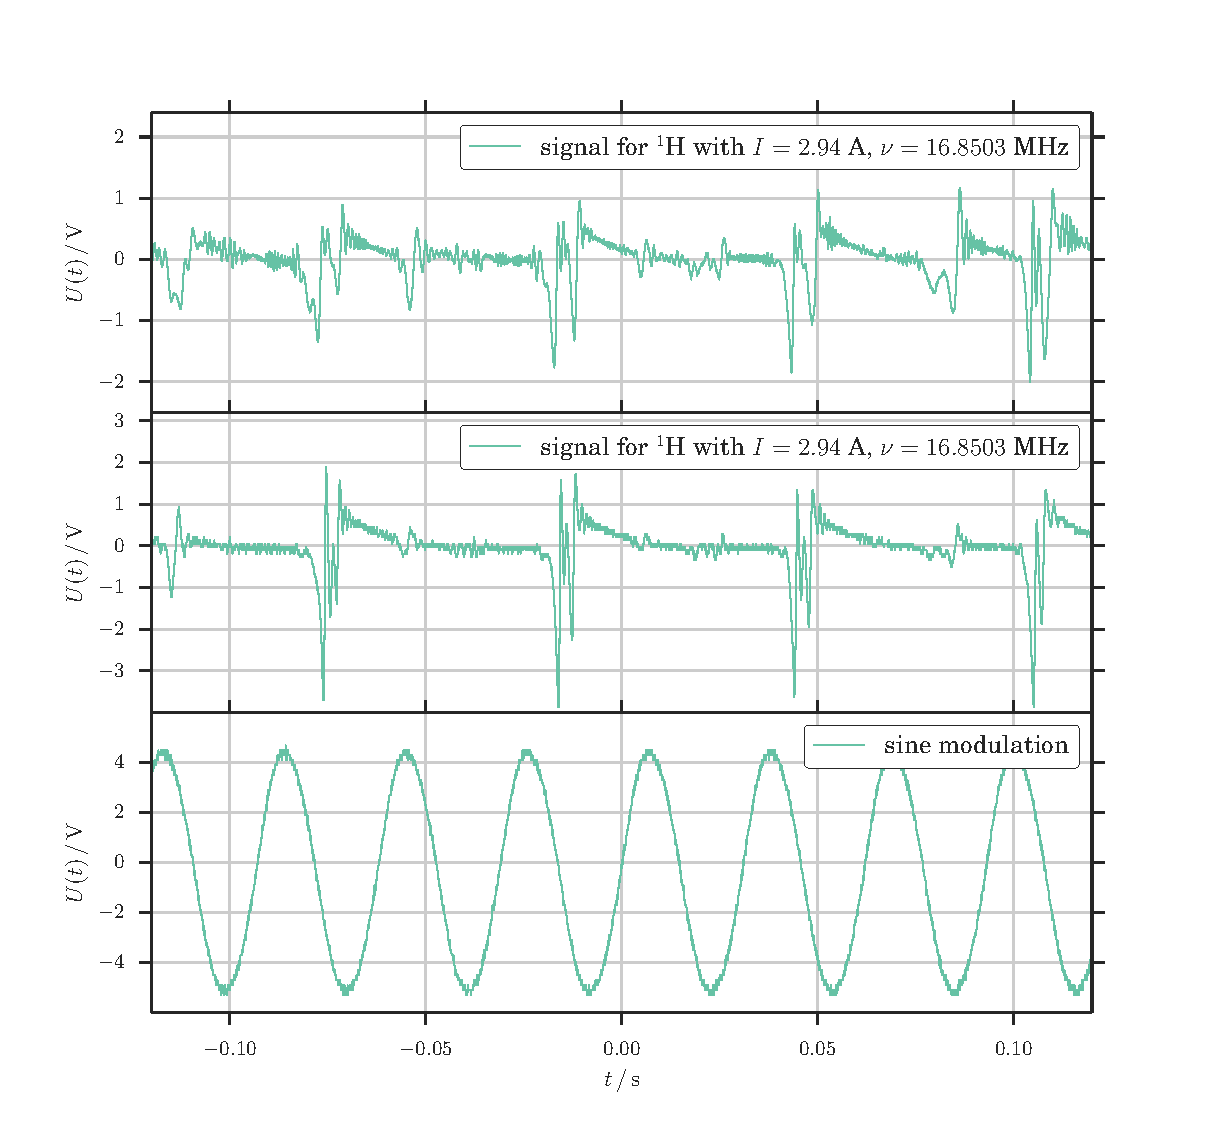
\includegraphics[width=\textwidth]{figures/f_r_H.pdf}
	\caption{
		Absorption peaks of proton ($^1$H) in water
		at two times, both with $B_\mathrm{measured} = 395$ mT.
		No equidistant absorption peaks at the zero intersect of the sine are seen.
		}
	\label{fig:f_r_H}
\end{figure}

\begin{figure}
	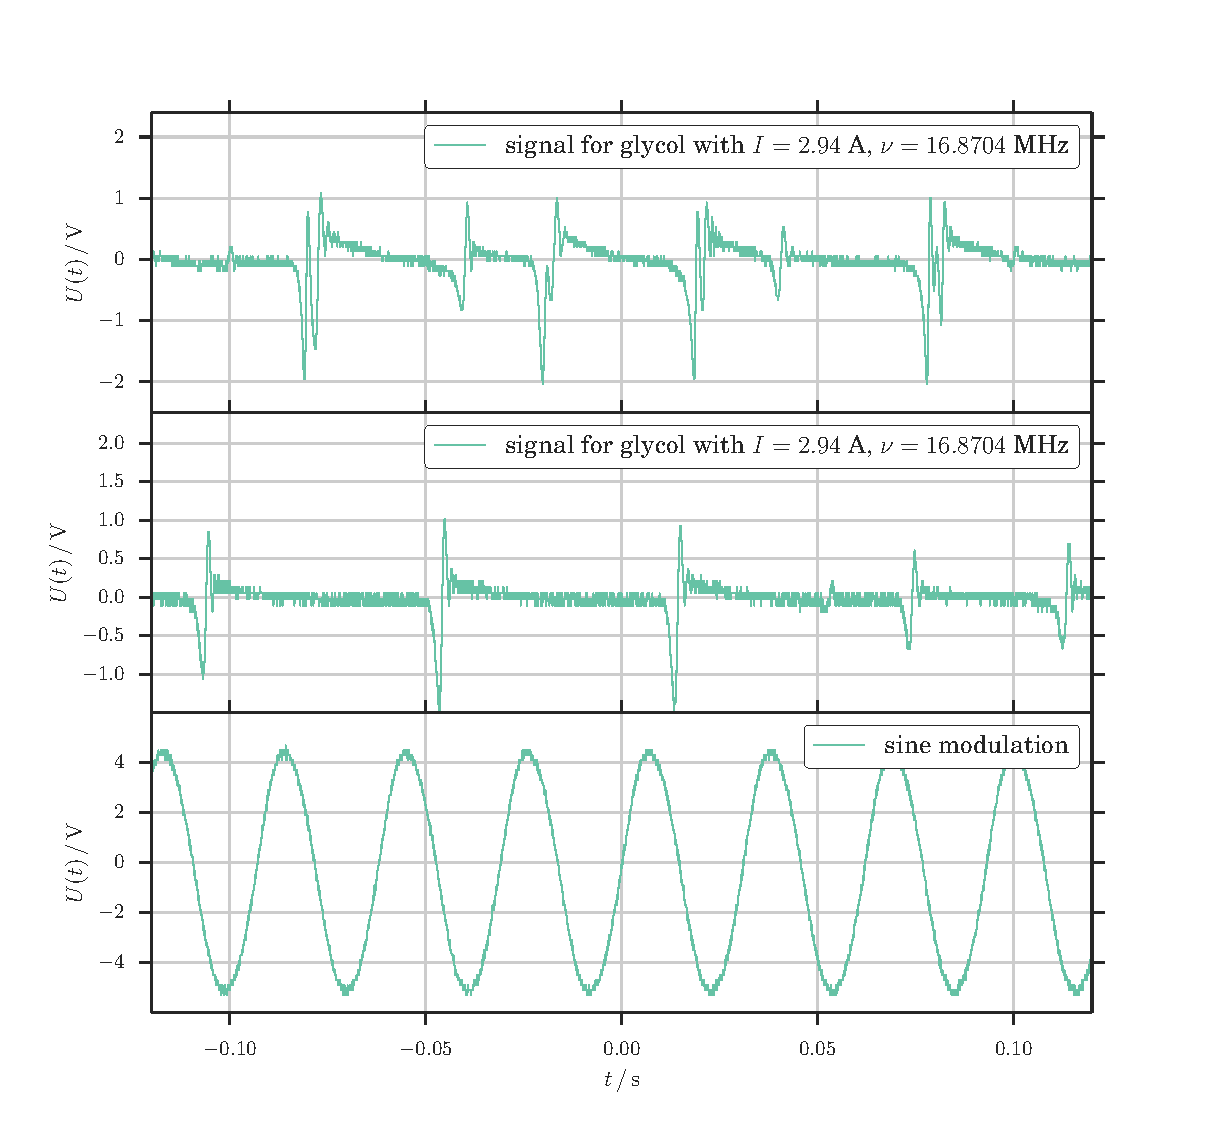
\includegraphics[width=\textwidth]{figures/f_r_glycol.pdf}
	\caption{
		Measured absorption peaks of proton ($^1$H) in glycol
		at two times, both with $B_\mathrm{measured} = 394$ mT.
		Again, no equidistant absorption peaks at the zero intersect of the sine are seen.
		}
	\label{fig:f_r_glycol}
\end{figure}


\FloatBarrier

\subsection{Measurements with lock-in method}
\paragraph{The measurement with}
the lock-in failed. we were not able to observe the expected signal 
after dedicating an entire day for this part of the experiment. We will, however document some 
of the calibration to illustrate the results of the theoretical section about the lock-in method 
and to possibly identify mistakes we made. 
We started the calibration by setting up the HF-generator and the main coil's magnetic field 
for the $^1$H sample such that a resonance signal could be observed as in the previous section.
This was achieved for a frequency of $\nu = 16.8220$ MHz and a current $I = 2.96$ A. 
The sine modulator's signal was set to the frequency of the one in the previous section, 
namely $31.9 \pm 1.0$ Hz, as can be obtained graphically by the period of $3T = (0.094 \pm 0.003)$ s 
of the rectangular signal in figure \ref{fig:phase}. Calculating the frequency from the 
oscilloscope's signal is necessary since the display of the sine generator was broken. 
We then analysed the phase difference between the sine modulation and the rectangular gate 
for the integration. The first part of this calibration was done by eye, observing the 
signal of the lock-in analyser without integration. The results are displayed in the figure
\ref{fig:phase}. As can be observed, for $T = 0$, the phase difference $\Delta \phi$ is not zero. 
Since we want to integrate the signal, we need to have a phse difference close to $\Delta \phi = n \pi$, 
$n \in \mathbb{N}$. We thus set the potentiometer 'Time const' to $T = 5.00 \pm 0.03$ with the 
toggles set to $T_\mathrm{step} = 25$ ms, Mode = Norm and $T_0$ = Norm. For integration, we 
chose a time span of 1 s. 
\begin{figure}
	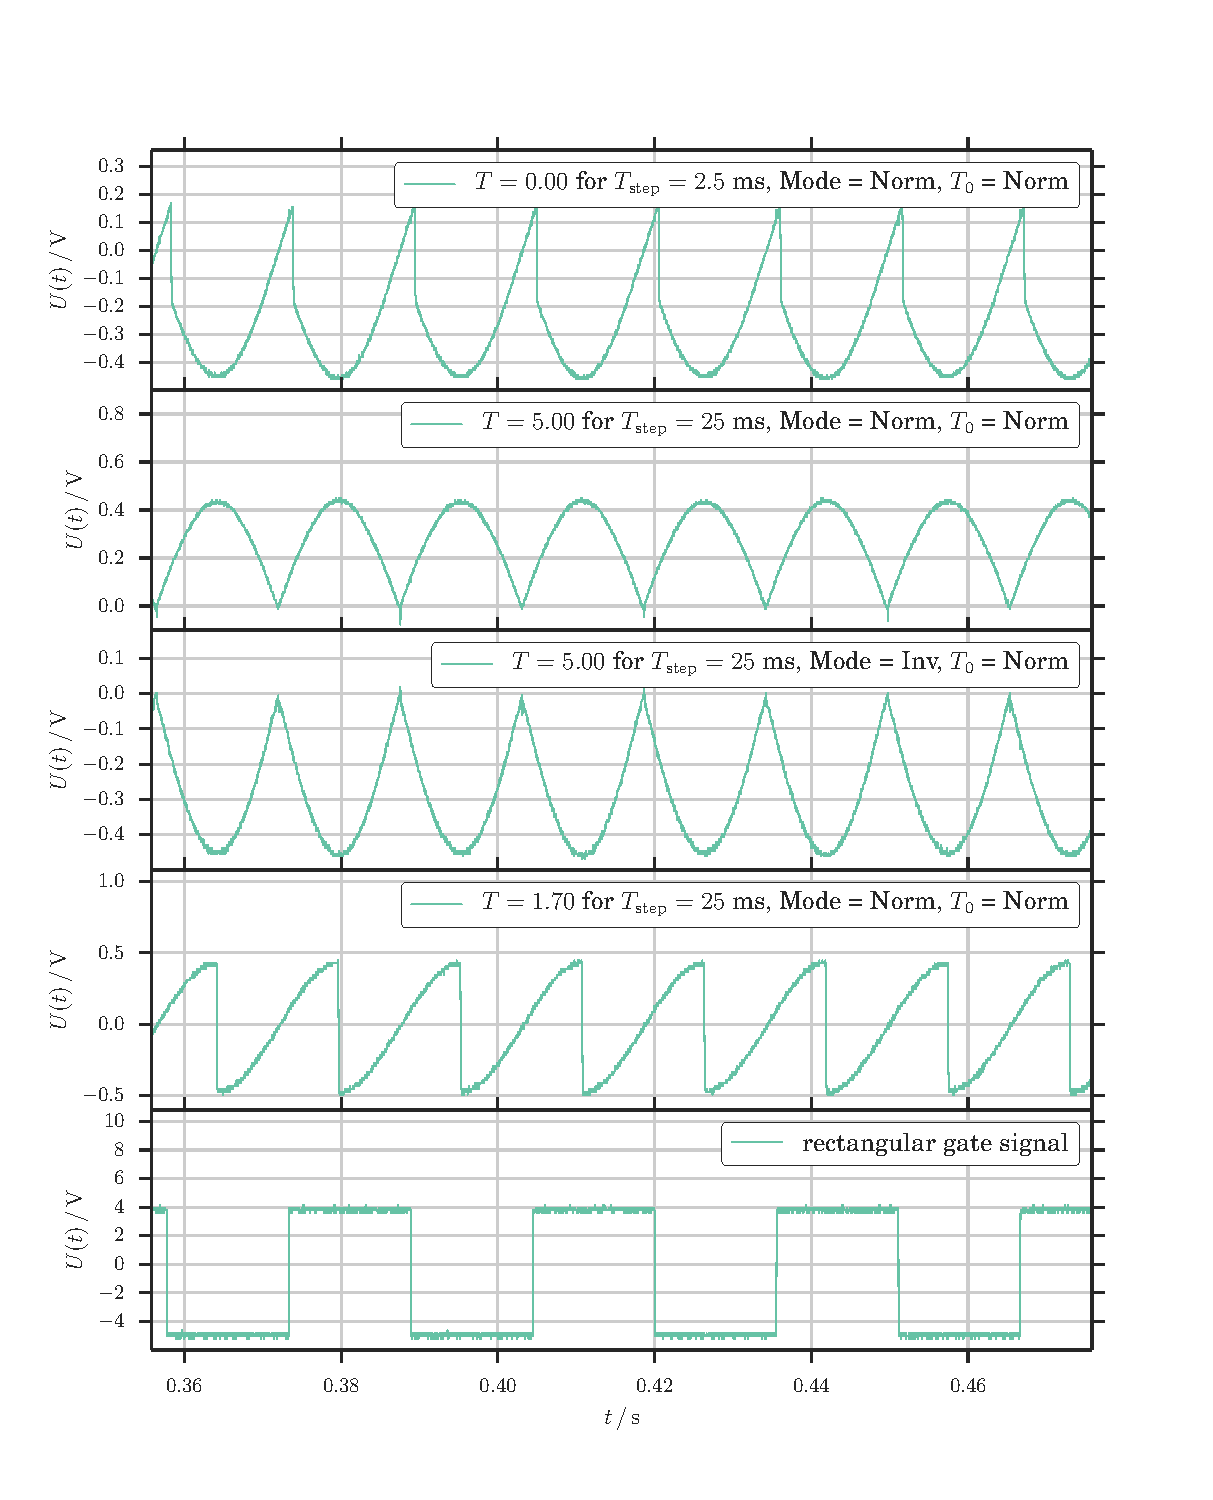
\includegraphics[width=\textwidth]{figures/phase.pdf}
	\caption{
		Lock-in phase calibration.
		$T$ indicates the value shown on the potentiometer 'Time Const', 
		the following three parameters correspond to the toggle switches located on the lock-in analyser.
		One can make the following observations: For $T = 0$, the phase difference $\Delta \phi$ is not zero;
		the inversion does not change the signal's form but only the sign; The phase differences corresponding 
		to the lower three signals are $\Delta \phi = 2\pi, \pi, \pi / 2$, respectively.
		The error on $T$ is given by $s_T = 0.03$.
		}
	\label{fig:phase}
\end{figure}



\paragraph{After completing the} 
phase calibration for the given frequency, we calibrated the 
sawtooth signal. We tried various values for the parameters available to configuration. 
However, with the given setup we did not observe any absorption peak as anticipated in the 
theoretical section. After some tries, we decided varying the frequency of the sine signal as 
well, again recalibrating the phase difference to $\Delta \phi = 2 \pi$ analogously.  
We given an example of the recorded data in figure \ref{fig:lock_in_example}, where we show 
the sine modulated sawtooth for $T_\mathrm{sawtooth} = 30$ s for a range of $t \in [0, 2] s$ and
over the entire time span $t \in [-30, 30]$, as well as 
the measured signal, basically consisting of noise. The frequency can again be calculated 
by reading of the period from the first graph:
\begin{align}
    32T  &= \left((1.97 - 0.00) \pm 0.02\right) \, \mathrm{s} \\
        &= (1.97 \pm 0.02) \, \mathrm{s} \\
    \Rightarrow \qquad f_\mathrm{sine} &= \frac{32}{32T} = 16.24 \mathrm{Hz} \\
    s_{f_\mathrm{sine}} &= \frac{32}{(32T)^2} s_{32T} = 0.16 \mathrm{Hz} \, .
\end{align}
The signal did not differ substantially from the one shown in the example. We thus have to 
relinquish from calculating the desired quantities from this method. 
\begin{figure}
	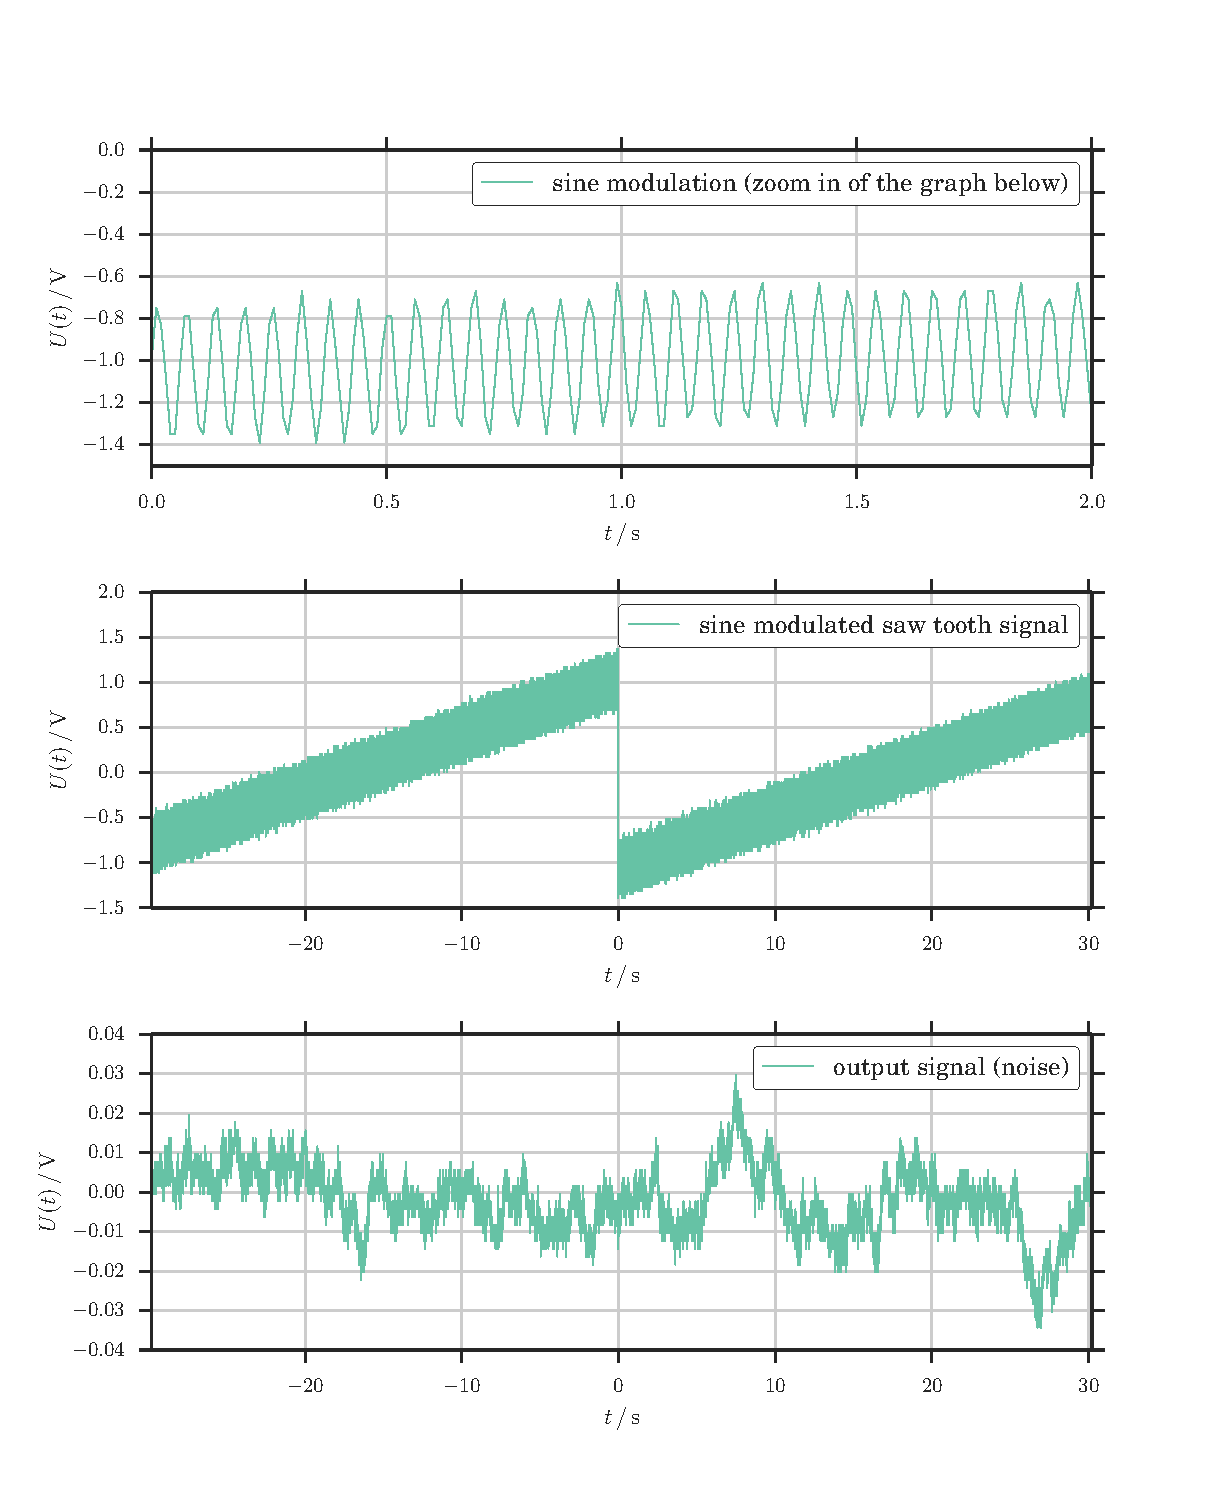
\includegraphics[width=\textwidth]{figures/example.pdf}
	\caption{
		Example for failure of the lock-in method.
		The upper two graphs show the sine modulated saw tooth signal
		in two different ranges for $t$. The zoomed range of the uppermost 
		graph can be used to calculate the frequency of the sine modulation.
		The output signal is basically noise, no absorption signal can be observed.
		}
	\label{fig:lock_in_example}
\end{figure}


\FloatBarrier
